\tikzstyle{service} = [rectangle, minimum width=2cm, text width=1.9cm, minimum height=1cm, text centered, draw=black, fill=white]
\tikzstyle{extservice} = [rectangle, minimum width=2cm, text width=1.9cm, minimum height=1cm, text centered, draw=black, fill=gray!50]
\tikzstyle{flow} = [thick,->,>=stealth]
\tikzstyle{depends} = [thick,-,>=stealth]

\chapter{System Architecture\label{chap:system-architecture}}
  \begin{figure}[!h]
    \centering
    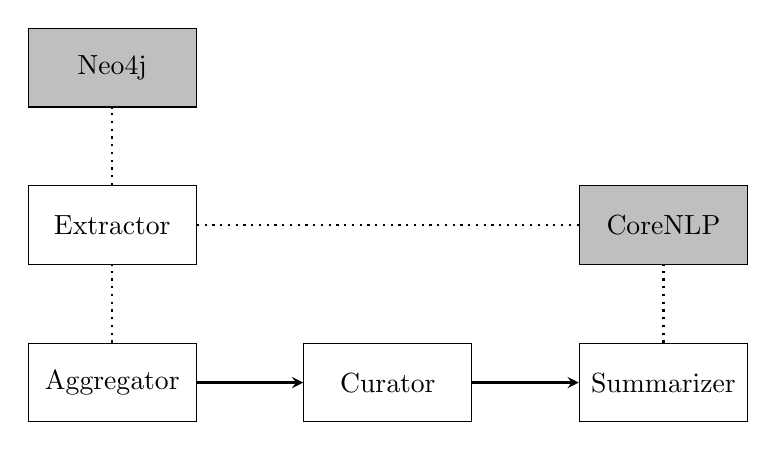
\begin{tikzpicture}[node distance=3.5cm]
      \node (agg) [service] {Aggregator};
      \node (ext) [service, above of=agg, yshift=-1.5cm] {Extractor};
      \node (cur) [service, right of=agg] {Curator};
      \node (sum) [service, right of=cur] {Summarizer};
      \node (cor) [extservice, above of=sum, yshift=-1.5cm] {CoreNLP};
      \node (neo) [extservice, above of=ext, yshift=-1.5cm] {Neo4j};

      \draw [flow] (agg) -- (cur);
      \draw [flow] (cur) -- (sum);
      \draw[dotted] [depends] (agg) -- (ext);
      \draw[dotted] [depends] (ext) -- (neo);
      \draw[dotted] [depends] (ext) -- (cor);
      \draw[dotted] [depends] (sum) -- (cor);
    \end{tikzpicture}
    \caption{\\Architecture Diagram. Arrows represent the pipeline; dotted lines represent dependencies.}
  \end{figure}
